Una vez estimada la planificación temporal y el presupuesto del proyecto, es momento de definir correctamente los requisitos y la funcionalidad que ofrecerá el producto. Para ello, haremos un análisis de requisitos del problema, estableceremos sus casos de uso y diseñaremos las clases y métodos necesarios durante la implementación. Finalmente, diseñaremos los bocetos del sitio web que próximamente daremos vida.

\section*{Análisis de requisitos}

Tras un estudio profundo del problema y evaluando la viabilidad de los mismos, introducimos los requisitos, funcionales y no funcionales, de este proyecto:

\subsection*{Requisitos funcionales}
En caso de la visualización de fractales 2D:
\begin{itemize}
    \item \textbf{RF1.1}: Visualización de conjuntos de Julia y Mandelbrot 2D.
    \item \textbf{RF1.2}: Posibilidad de alternar qué fractal ver en el canvas: Julia o Mandelbrot.
    \item \textbf{RF1.3}: Posibilidad de cambiar el exponente $m$ de la función $P_{c,m}(z)=z^m+c$ para poder visualizar conjuntos de Julia y Mandelbrot generalizados.
    \item \textbf{RF1.4}: Posibilidad de cambiar la constante $c$ de la función $P_{c,m}(z)=z^m+c$ en el caso de los conjuntos de Julia para poder visualizar diferentes conjuntos de Julia $\mathcal{J}_c$ para distintos $c\in\C$.
    \item \textbf{RF1.5}: Poder movernos libremente por el plano.
    \item \textbf{RF1.6}: Hacer zoom de forma que podamos observar las infinitas irregularidades que presentan los fractales.
    \item \textbf{RF1.7}: Modificar los parámetros que acepten los algoritmos utilizados para visualizar los fractales para ver cómo cambia la imagen al cambiar dichos parámetros.
\end{itemize}
En caso de fractales 3D:
\begin{itemize}
    \item \textbf{RF2.1}: Visualización de generalizaciones tridimensionales de los conjuntos de Julia y Mandelbrot.
    \item Posibilidad de alternar qué fractal ver en el canvas en cada momento.
    \item \textbf{RF2.2}: Posibilidad de modificar parámetros del modelo de iluminación para así observar distintos materiales y coloraciones en los fractales.
    \item \textbf{RF2.3}: Modificar parámetros de los algoritmos de visualización que empleemos.
    \item Posibilidad de moverse libremente por la escena utilizando una cámara orbital.
    \item \textbf{RF2.4}: Hacer zoom en la escena para poder observar de cerca las superficies de los fractales.
\end{itemize}
De forma genérica:
\begin{itemize}
    \item \textbf{RF3}: Botón de reseteo para restablecer los valores de los parámetros por defecto.
    \item \textbf{RF4}: Posibilidad de cambiar rápidamente entre visualización 2D y 3D.
\end{itemize}

\subsection*{Requisitos no funcionales}

\begin{itemize}
    \item \textbf{RNF1}: El tiempo de procesado no debe ser demasiado largo. A ser posible se ejecutará en tiempo real.
    \item \textbf{RNF2}: Deben utilizarse herramientas portables, es decir, que puedan ejecutarse en cualquier navegador sin necesidad de instalar nada.
    \item \textbf{RNF3}: La interfaz de usuario tiene que ser sencilla, para que pueda utilizarla cualquier persona.
    \item \textbf{RNF4}: El software debe poder ser ejecutado en cualquier ordenador estándar. Por tanto, las técnicas utilizadas no pueden requerir un hardware demasiado avanzado ni demasiado caro.
    \item \textbf{RNF5}: Es necesario incluir cierta documentación en la web para que el usuario con pocos conocimientos sepa identificar el uso de cada parámetro.
    \item \textbf{RNF6}: Deben usarse colores e interfaces que cuiden la experiencia de usuario.
    \item \textbf{RNF7}: No será posible elegir valores de parámetros imposibles o que requieran una cantidad inviable de cálculo.
\end{itemize}

\subsection*{Requisitos de datos}

No existen requisitos de datos, ya que no hay realmente ninguna base de datos ni es necesaria, pues no es una aplicación que almacene datos, sino que realiza cálculos para graficar imágenes.

\section*{Análisis de casos de uso}

A continuación describiremos los posibles casos de uso del software a desarrollar:
\begin{itemize}
    \item \textbf{CU1}: Primer acceso a la página. El usuario accede por primera vez a la página.
    \item \textbf{CU2}: Modificar un parámetro. El usuario cambia uno de los distintos parámetros modificables.
    \item \textbf{CU3}: Comprobar si un nuevo parámetro es incorrecto o inviable. Ante el cambio de un parámetro, es necesario comprobar que no se ha introducido un valor imposible o computacionalmente inviable. Por ejemplo, un número negativo o demasiado grande de iteraciones.
    \item \textbf{CU4}: Web sobrecargada. Posible sobrecarga provocada por una excesiva demanda de cálculo en poco tiempo.
    \item \textbf{CU5}: Establecer valores por defecto. Cambiar los parámetros de la escena a los que se toman por defecto.
    \item \textbf{CU6}: Dibujar la escena. Visualizar la escena a partir de los parámetros actuales, estando seguros de que son correctos.
    \item \textbf{CU7}: Mensaje de error. Ante cualquier error posible, se notifica del mismo al usuario.
\end{itemize}

Ante estos casos de uso, en la figura \ref{fig:casos-uso} vemos el diagrama de casos de uso, en el cual vemos a cuales de ellos puede acceder el usuario y qué interdependencias hay entre ellos.

\begin{figure} [ht]
\centering
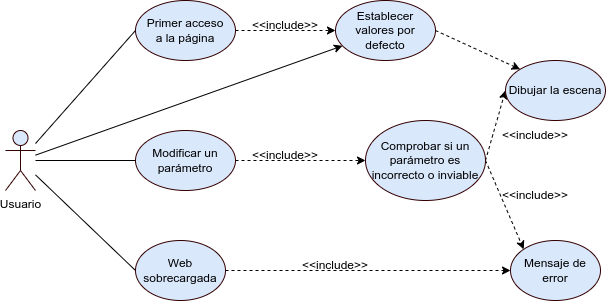
\includegraphics[scale = 0.6]{img/diagrama-CU.png}
\caption{Diagrama de Casos de Uso}
    \label{fig:casos-uso}
\end{figure}
\newpage
\section*{Bocetos de la web}

A continuación presentaremos los bocetos básicos, a veces llamados `wireframes', de la apariencia que tendrá la web. Son únicamente tres pantallas, y dos de ellas son prácticamente iguales en lo que a nivel de boceto se refiere. La pantalla en la que se visualizan fractales 2D y 3D en un canvas (imagen \ref{fig:wireframe-fractals}) es prácticamente igual en ambos casos, por lo que sólo hemos incluido una de ellas entendiendo que los enlaces y los títulos son intercambiables en cada versión. 

\begin{figure} [ht]
\centering
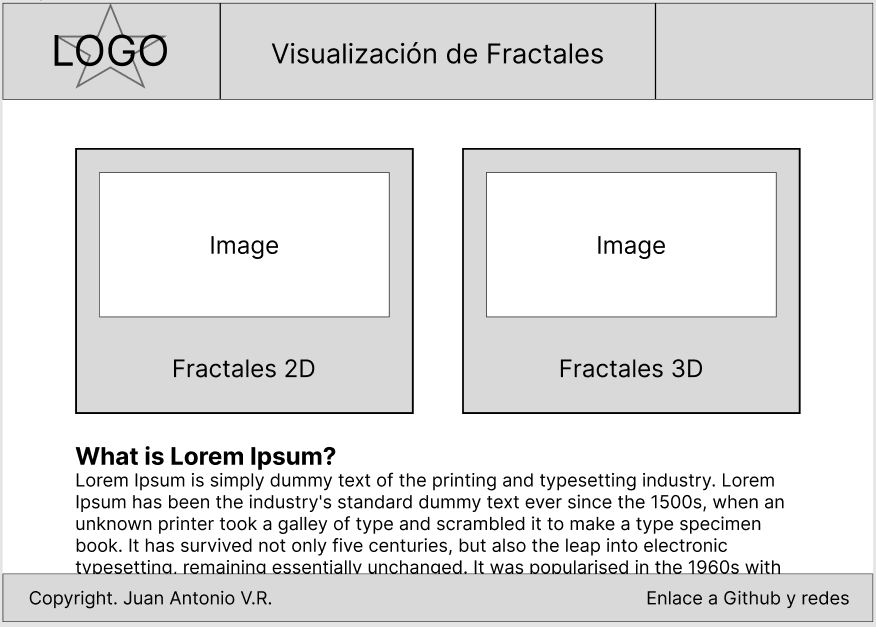
\includegraphics[scale = 0.4]{img/wireframe-home.png}
\caption{Wireframe de la portada de la página}
\label{fig:wireframe-home}
\end{figure}

Como vemos en la imagen \ref{fig:wireframe-home}, al acceder a la web nos aparecería la posibilidad de elegir si queremos explorar el mundo de los fractales 2D o 3D. Debajo del menú seleccionable aparecería una breve introducción al mundo de los fractales desde un punto de vista entendible por casi cualquier persona.

\begin{figure} [ht]
\centering
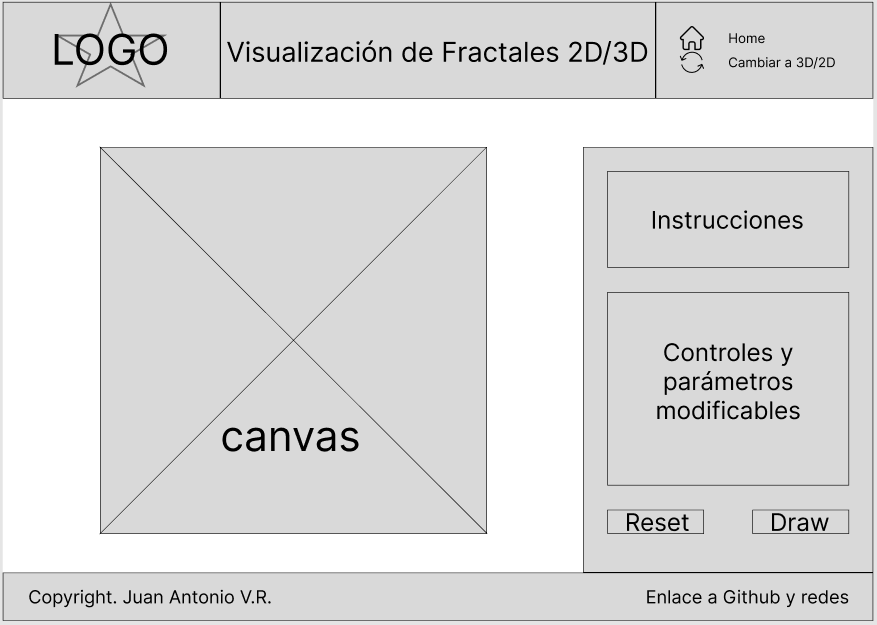
\includegraphics[scale = 0.4]{img/wireframe-1.png}
\caption{Wireframe de la pantalla en la que se visualizan fractales}
    \label{fig:wireframe-fractals}
\end{figure}

Sobre la pantalla de la imagen \ref{fig:wireframe-fractals}, aparecería a la izquierda el canvas donde se visualizarían los fractales y los distintos controles y parámetros modificables estarían en el lado derecho. Debajo de esta sección de la pantalla también se incluiría un texto documentando el sentido de cada parámetro para que el usuario que no conozca demasiado el trasfondo matemático ni informático pueda interactuar sin problemas.